\chapter{Literature review}
\section{Introduction}
This chapter aims to provide an overview and foundation of the current knowledge of this study in literature as well as a theoretical base for the work done in this study. Fundamentals pertaining to this study are presented. The solution techniques related to \acrshort{afff} have been proposed and analysed by many researchers. All optimization problems are about maximizing the effectiveness and efficiency of \acrshort{afff}. Inputs and outputs of these solution techniques have different limitations and difficulties which lead researchers to propose ideas about finding the best solution to these techniques.

The first section of the literature is a brief overview of significant fundamentals of \acrshort{afff}-focusing on the evolutionary changes, characterization, foaming ability, mechanical stability, and critical application rates. This is followed by a review and analysis of current problems and difficulties based on the optimization of \acrshort{afff}. Issues concerning the compatibility of various storage facilities on \acrshort{afff} are discussed. Previous studies and experimental work aiming at the optimization of \acrshort{afff} are discussed.

\section{A brief overview of various firefighting foams}
In the aviation industry, fire is of great concern due to the incidences of fires that are usually devastating to both human lives and properties. Since fire is of great significant in the present research, it is beneficial to understand various classes of fire. Fire is usually classified in five (5) classes. In fire science, fire is classified by the type of fuel they burn namely: Class A, B, C, D, and K. \cite{oguike2013study}.  The classes are discussed in detail in Table \ref{ch2:table:classes}. However, the present research work will only focus on Class B fire, since \acrshort{afff} is utilised to suppress this Class of fire.

\begin{table}[H]
\onehalfspacing
\centering
\caption{Various classes of fire \cite{hinnant2020characterizing}.}
\begin{tabularx}{\textwidth}{ >{\hsize=.45\hsize}X >{\hsize=1.35\hsize}X >{\hsize=.9\hsize}X }
\hline
Class of fire & Type of fire & Commonly encountered \\ 
\hline
A & Common combustibles such as wood, paper, and rubber materials. & General places. \\
B & Flammable liquids such as fuel, petroleum greases, and flammable gases. & Airports and petroleum industries. \\
C & Energized electrical equipment and conductors. & Electrical distribution industries. \\
D & Combustible metals such as magnesium, titanium, and sodium. & Metal manufacturers. \\ 
K & Cooking oils, normal grease, and animal fat. & Production and FMCG industries. \\
\hline
\end{tabularx}
\label{ch2:table:classes}
\end{table}

In the aviation industry, firefighting foam was declared by \acrshort{faa} as the sole optimal extinguishing medium used for suppression of Class B fire during emergency conditions. Originally, five types of firefighting foams are commonly used: \acrfullpl{fp}, \acrfullpl{afff}, \acrfullpl{fffp}, \acrfullpl{ar-afff} and \acrfullpl{ar-afffp} \cite{george2002introduction}. All of them were designed to be effective in handling precise fire conditions and contain one or more fluorinated surfactants as a key ingredient.

In general, foam is made by first mixing foam concentrate with water to create a foam solution. This aqueous solution is then blended with air using standard aspirating nozzles to generate foam \cite{george2002introduction}.  Fire-fighting foam is an extinguishing agent composed of numerous bubbles formed mechanically or chemically from the liquid, as shown in Figure \ref{ch2:figure:scheme}. These are commonly used to reduce the spread and extinguishing of Class B fires and to prevent re-ignition whilst in certain situations may be implemented to extinguishing Class A fires \cite{oguike2013study}. Sometimes capabilities of firefighting foams can be reduced due to ignorance. Hence foam may be assumed to have performance concerns, whereas it does not. 

\begin{figure}[H]
    \centering
    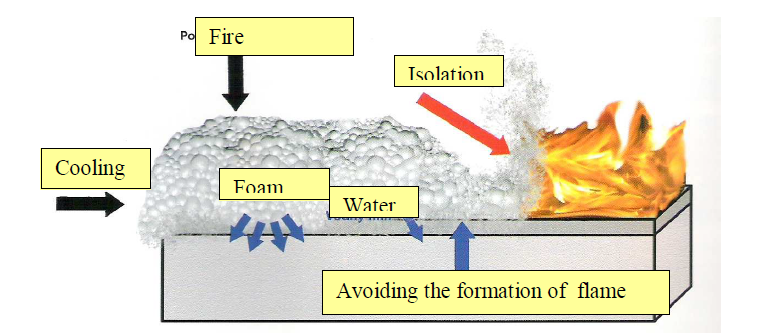
\includegraphics[width=.8\textwidth]{extinguishing_mechanism_scheme.png}
    \caption{Scheme of the extinguishing mechanism by using firefighting foam \cite{turekova2011environmental}}
    \label{ch2:figure:scheme}
\end{figure}

\section{Evolution of AFFF for effective extinguishment of Class B fires}
Water has long been a universal agent for suppression of fires, however, it is not exceptional in all instances \cite{hinnant2020characterizing}. For instance, water is regularly incapable of suppressing combustible fluids and can be perilous. Protein-based foams which presented a drastic improvement over water for combating liquid fuel fires were developed and used initially. These protein-based foams are thick and form a heavy, heat-resistant covering over a burning liquid surface \cite{scheffey1995evaluating}. These properties made protein-based foams to be constrained as they were not able to spread rapidly over the fuel surface. This was a concern for a long time, as protein-based foams were not much effective in low viscosity fuels such as kerosene that is commonly used in aviation industry. The ineffectiveness was due to the inability of protein-based foams to spread rapidly.

Synthetic based foams were developed and introduced in the mid-1960s to optimize protein-based foams \cite{aamodt2020review} . These firefighting foams included \acrshort{afff} and \acrshort{ar-afff}. They generally provide better flow and spreading over the burning fuel surface, for faster knockdown of flames. \acrshort{afff} concentrates are made from blending fluoro-and hydrocarbon-surfactant, modest quantities of salts and foam stabilizers are regularly included \cite{wang2019research}. The \acrshort{afff} concentrate is then mixed with a specific level of water to form a foam solution. The proportioning rate is usually, 1\%, 3\% and 6\% of foam concentrate to water. Furthermore, an additional feature of 'aqueous film' is formed on the surface of a flammable liquid by the foam solution as it drains from the foam blanket \cite{hinnant2020characterizing}. This film is very fluid and floats on the surface of most hydrocarbon fuels, hence providing \acrshort{afff} with tremendous speed during extinguishing conditions. This made \acrshort{afff} to be further developed and predominant to most firefighting foams. Moreover, the introduction of \acrshort{afff} represented a significant increase in firefighting performance in terms of more rapid control and extinguishment of fuel fires, especial in industries that are involved with low viscosity fuels. The vital chemical composition of \acrshort{afff} are depicted in Table A.1 on appendices.

It is essential to comprehend that Class B fires are exothermic reaction that relies significantly upon four (4) elements: fuel, air/oxygen, heat, and chemical chain reaction \cite{beneventi2001role}. Removing one element will effectively halt the fire.  However, all firefighting foams do not interfere with the chemical reaction when extinguishing fuel fires, yet four (4) suppression mechanisms are required for knockdown and burn-back resistance:

\begin{itemize}
    \item The foam blankets the fuel surface smothering the fire. 
    \item The foam blanket separates the flames/ignition source from the fuel surface. 
    \item The foam cools the fuel and any adjacent metal surfaces. 
    \item The foam blanket suppresses the release of combustible fumes that can mix with air \cite{beneventi2001role}. 
\end{itemize}

All firefighting foams were developed for suppression of specific combustible fuels. It is vital to identify which fuel group is involved when flammable fire conditions occur. This is to ensure timeous and effective extinguishment during fire conditions. As a consequent, firefighting foam may be ineffective when used on unsuitable fuel, hence may yield unexpected or unfavorable outcomes. There are two different basic flammable or combustible fuel groups:

\begin{itemize}
    \item Standard hydrocarbon fuels such as gasoline, diesel, kerosene, jet fuel etc. these fuels do not blend with water or are not miscible in water, they usually float on top of water and, for the most part, they do not intermix.
    \item Polar solvent or Alcohol type fuels are fuels that mix readily with water or are miscible in water \cite{beneventi2001role}.
\end{itemize}

To date, \acrshort{afff} has been widely used in aviation fire protection for suppression of hydrocarbon fuels (a part of Class B fires). This synthetic based foam has a low viscosity and spreads quickly across the surface of most hydrocarbon fuels. Initially, \acrshort{afff} was developed for aviation industries due to the fuel (kerosene) they are involved with and have proven to be effective in several cases. However, they can also be relatively utilized for extinguishing Class A fires. During firefighting a water film forms underneath the foam, which cools the liquid fuel, halting the formation of combustible fumes \cite{scheffey1995evaluating}. Consequently, this gives a sensational fire knockdown, which is a critical aspect in crash rescue firefighting.

\section{Foam generating process}
Foam, in general, is created by a mechanical action (dispensing equipment), hence the generation of firefighting foam is a mechanical process that comprises numerous prior steps. There are various methods of generating firefighting foam, each method relies on the class of fire involve and foam solution used. To date, there are three (3) methods of generating firefighting foam from a foam solution namely: aspirated nozzle, \acrfull{caf}, and chemical reaction method \cite{laundess2012suppression}. The distinctions in these methods yield unique characteristics of foam produced with noticeable contrasts being the size and uniformity of the bubbles produced using each method \cite{laundess2012suppression}. Such differences may lead to significant variation of foam performance during fire conditions. However, the aspirated nozzle is a traditional and widely used method of generating firefighting foam, particularly in aviation fire protection.

Aviation fire protection have adopted the technique of aspirated nozzle when generating foam. This technique is more useful for aviation fire protection due to the type of environment and aviation standards that were developed and led by the \acrfull{nfpa}. Technically and according to the research, the aspirated nozzle is suitable for low expansion foams such as \acrshort{afff} and \acrshort{ar-afff} \cite{xi2017experimental}.  Aviation fire protection utilizes \acrshort{afff} for fire suppression due to the class of fuel (Jet A-1) they are involved with. Subsequently, the aspirated nozzle technique has been compatible with \acrshort{afff}. However, during the periodic tests in aviation, the functionality of this technique is tested and according to the reports, there are still concerns when using it \cite{laundess2012suppression}. Moreover, the gaps exist in the optimization of this foam generation.

Comprehending of various foam generation methods is essential in the present research work in order to evaluate and deduce if any other method can yield any benefits. Most Research have been focusing on the aspirated nozzle and \acrshort{caf} generation methods aiming to optimize or implement new methods. Optimization of these methods require complex mathematical analysis as there are numerous parameters involved. Besides, the complexity further relies on the variation of chemicals involved in the chemical reaction technique.

In the present study, the aspirated nozzle technique is evaluated against \acrshort{caf} and chemical reaction methods in order to minimize or eliminate the optimization challenges of this foam generation method in aviation fire protection. The experimental work conducted by Laundess et al \cite{laundess2012suppression} shows that foam generated by \acrshort{caf} technique displays uniformly small size bubbles, aspirated nozzle produces a greater spread of bubble sizes while chemical (nitrogen) reaction displays most uniform size distribution of bubbles as shown in Figure \ref{ch2:figure:characteristics}. In addition, the \acrshort{caf} method has the advantage of being environmentally friendly.  With the aspirated nozzle technique having environmental concerns, a new technique or optimization has emerged as an alternative in aviation fire protection.

\begin{figure}[H]
    \centering
    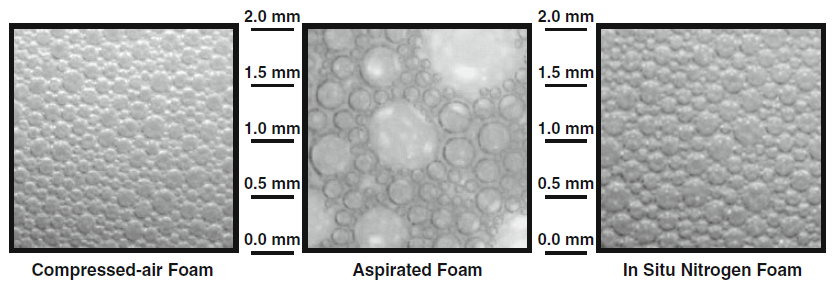
\includegraphics[width=.95\textwidth]{bubble_characteristics.png}
    \caption{Bubble characteristics for different generation methods \cite{laundess2012suppression}.}
    \label{ch2:figure:characteristics}
\end{figure}

\subsection{Aspirated nozzle}
The technique has been extensively used and is the traditional way of generating firefighting foam. In this method, foam is generated by extracting air into a jet of foam solution inside a nozzle \cite{xi2017experimental}. Most firefighting foam nozzles are specially designed in a convergent geometry. In this way, parameters such as pressure, velocity, and flow rate are carefully controlled as shown in Figure \ref{ch2:figure:nozzle}, foam solution at high pressure and low velocity enters the orifice at 1 and exit as finished foam at low pressure and high velocity at 5, at a constant flow rate. During stages 2, 3, and 4 air is drawn by a jet and blended with foam solution resulting in a strong mixing and agitation \cite{csb2016phenomenological}.

\begin{figure}[H]
    \centering
    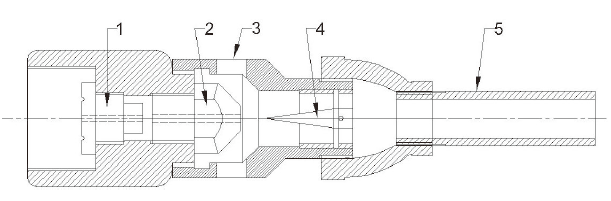
\includegraphics[width=\textwidth]{foam_generating_nozzle.png}
    \caption{Nozzle for generating foam \cite{csb2016phenomenological}.}
    \label{ch2:figure:nozzle}
\end{figure}

The governing equation for critical parameters during the foam generation is usually the Bernoulli's equation, which is given as:

\begin{equation}
    P_1+\frac{1}{2}\rho{v_1}^2 + \rho gh_1 = P_5+\frac{1}{2}\rho{v_5}^2 + \rho gh_5
\end{equation}

As seen in Figure \ref{ch2:figure:nozzle}, in case where the potential energy at the elevation 1 ($\rho gh_1$) equals the potential energy at elevation 2 ($\rho gh_5$), then the equation can be simplified and written as:

\begin{equation}
    P_1+\frac{1}{2}\rho{v_1}^2 = P_5+\frac{1}{2}\rho{v_5}^2
\end{equation}

\begin{doublespace}
    Where, \\
    $p_1\ is\ the\ pressure\ at\ elevation\ 1\ in\ Pa$ \\
    $v_1\ is\ the\ velocity\ at\ elevation\ 1\ in\ m/s$ \\
    $h_1\ is\ the\ height\ at\ elavation\ 1\ in\ m$ \\
    $P_5\ is\ the\ pressure\ at\ elavation\ 2\ in\ Pa$ \\
    $v_5\ is\ the velocity\ at\ elavation\ 2\ in\ m/s$ \\
    $h_5\ is\ the\ height\ at\ elevation\ 2\ in\ m$ \\
    $g\ is\ the\ acceleration\ due\ to\ gravity\ in\ m/s^2$ \\
    $\rho\ is\ the\ density\ of\ fuid\ in\ kg/m^3$ \\
\end{doublespace}

Since convergent nozzles are used to increase the outlet velocity ($v_5$  in figure \ref{ch2:figure:nozzle}) due to the conservation of mass, while critically maintaining the inlet flowrate during firefighting. Therefore, the following assumptions can be made:

\begin{gather*}
    A_1 > A_5 \\
    V_1 > V_5 \\
    P_1 > P_5
\end{gather*}

When the areas of the inlet and outlet are known and the flow rate that must be achieved is also known, then velocities can be calculated using the following equation:

\begin{equation}
    Q = VA
\end{equation}


\begin{doublespace}
    Where, \\
    $Q\ is\ the\ flowrate\ in m^3/s$ \\
    $V\ is\ the\ velocity\ of\ foam\ solution in m/s$ \\
    $A\ is\ the\ area\ of\ the\ nozzle\ at\ a\ particular\ point\ in\ m^2$ \\
\end{doublespace}

Over the years, researchers have been focusing on the source of these problems in order to comprehend the mathematical difficulties involved. However, engineers have been working on mathematical solution techniques in order to optimize convergent foam nozzles in aviation fire protection. Aspirated nozzle problems are noticeable during periodic trainings and uncertainty in the origination of the problem is mostly the challenge for many researchers.

\subsection{Compressed air foam (CAF)}
The \acrshort{caf} method is commonly used for generating any kind of firefighting foam and was developed initially by the \Acrfull{nrcc} in the late 1990s \cite{rie2016class}. The technique has offered several benefits in fire protection since the prohibition of halogen-based agents due to some environmental impacts.  

\acrshort{caf} technique is similar to the aspirated nozzle method as it also consists of a divergent nozzle for discharging foam. The distinction is that, in the \acrshort{caf} system, air is pressurized using an air compressor then fed or injected in an aqueous foam solution, as the foam expands its then discharges and guided through a nozzle.

\subsection{Chemical reaction}
This is a modern technique that was discovered by \cite{laundess2012suppression} to eliminate foam generation problems. The method has not yet been recognized in fire protection standards but certainly has several benefits. With other generation methods extensively used to produce much heavier carbon dioxide bubbles, it was of great practical significance to evaluate other methods that will produce lighter uniform bubbles. Consequently, nitrogen gas bubbles were the empirical and realistic alternative. In this way, the chemical reaction of foam solution and nitrogen creates numerous, uniformly sized bubbles of nitrogen gas within the foam.

The method has been reviewed by many researchers.  The only concern is the need to optimize foam formulations to prevent surfactants from being affected by the nitrogen generation and by the presence of salts formed during chemical reaction \cite{laundess2012suppression}.  For this reason, aviation fire protection will need to examine this as an alternative of possibly eliminating the aspirated nozzle method.

\section{Foaming ability and Mechanical stability}
Modern firefighting foams are primarily of the mechanical type. This means that before being utilized, they should be proportioned (mixed with water) and aerated (blended with air). Four elements are necessary to produce a quality and stable foam blanket and they include: foam concentrate, water, air, and aeration (mechanical agitation) \cite{oguike2013study}.

In recent years, mechanical stability has been a concern for most firefighting foams. Many researchers have approached this challenge with the aim of optimization. Foaming ability is a key process in advancing the mechanical stability of firefighting foams. Foam is a collection of air bubbles produced from a foaming solution \cite{oguike2013study}. The rate of this transformation is essential for evaluating the mechanical stability of the foam. Stability properties, as well as the effectiveness of firefighting foams, are determined by their physical and chemical properties, as described by Turekova and Balog \cite{turekova2011environmental}. These properties may include: the number of foaming, viscosity, foam frost resistance, the content of the sediment, foam stability, half-life of foam, pH, foaming solution of spreading factor \cite{turekova2011environmental}.

Synthetic based foams are low viscosity foams, consequently, they spread easily on the surface of the flammable liquid. This enables the formation of a dense and stable foam layer that acts as a physical boundary against the heat and mass transfer, thus exhibiting excellent cooling and covering effects in hydrocarbon fires \cite{xu2020fire}. The mechanical stability of \acrshort{afff} depends upon the structure of surface films from the so called-foaming agents. During firefighting conditions, the foams are continuously disrupted by the influence of heat of ignition, the internal force of foam, and the hot surface of burning liquid \cite{turekova2011environmental}. Foaming ability is thus a fundamental procedure as it directly affects the quality, hence the performance of the foam. The important parameters affecting a foam's ability to extinguish hydrocarbon fuel fire was addressed by Joseph et al \cite{scheffey1995evaluating} as shown in Figure \ref{ch2:figure:parameters}, with a theoretical modeling to further evaluate the challenges and limitation of the current methods used. 

\begin{figure}[H]
    \centering
    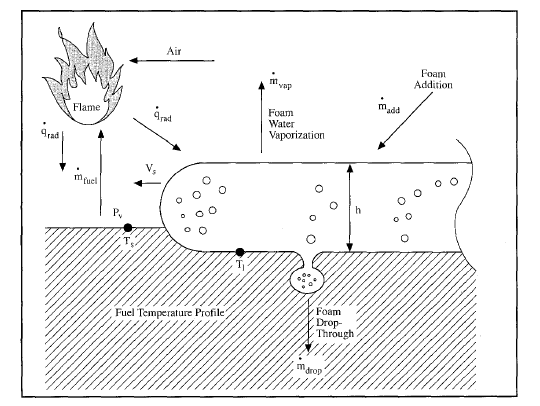
\includegraphics[width=\textwidth]{important_parameters.png}
    \caption{Important parameters affecting a foam's ability to exthinguishh hydrocarbon fuel fire \cite{scheffey1995evaluating}.}
    \label{ch2:figure:parameters}
\end{figure}

Oguike \cite{oguike2013study} conducted experimental tests intending to assess the foaming ability of various foams. The analysis comprised of eight (8) empty bottles, different volume of water was added and a constant foam concentrate was also added. The bottles were shaken vigorously at a steady time in each case and foam height was recorded. The foams were left to stand for some time and heights were measured again. Foams were left to stand for further days and height was measured again. Finally, foams formed were left to stand until collapse, and time was recorded for each foam solution. This experiment set a benchmark for most researchers, as most of the other foaming ability experiments have been based on it.

The current challenge is to develop small-scale test methods that measure these parameters in such a way that they can be used to predict large-scale foam performance. Persson \cite{persson1992fire} described optimization techniques and results to investigate foam mass loss by evaporation as a function of radiant heat from a fire. The finding was that foam viscosity and spreading is an area requiring further investigation. 

\subsection{AFFF blanket stability/drainage time}
Drainage time is often used to analyze the stability of various foams, however, it does not provide a reliable indication of the firefighting capability of foams. Drainage time is a measurement of the rate at which foam solution drains out of finished foam and hence provides an indication of the stability of the foam blanket \cite{aamodt2020review}. High expansion foams usually maintain the stability and heat resistance due to their long drainage time and hence slow loss of water from the finished foam. 

Since \acrshort{afff} is a low expansion foam, there are difficulties in maintaining the stability and heat resistance from the finished foam. This is due to short drainage time which indicates that finished foam losses its water content rapidly and renders it vulnerable to high-temperature flames and hot surfaces. A basic principle of measuring low expansion foam expansion ratios is shown in Figure \ref{ch2:figure:tests}. In recent years, most researchers concluded that the drainage times of finished foams do not solely depend on foam concentrate but also the type of foam generation \cite{martin2012fire}. In most cases, drainage time for low expansion foams such as \acrshort{afff} is often expressed as 25\% drainage time, while for medium and high it's usually 50\% drainage time. This is the time taken for 25\% or 50\% of the original foam solution content (by volume) to drain from the finished foam, as shown in Figure \ref{ch2:figure:tests}.

\begin{figure}[H]

\centering
\begin{subfigure}{.45\textwidth}
    \centering
    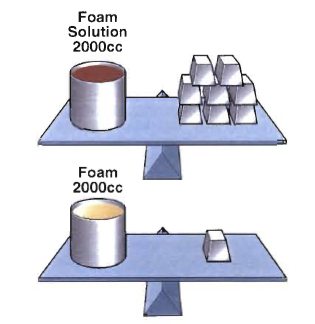
\includegraphics[width=\textwidth]{low_expansion_test.png}
    \caption{}
\end{subfigure}
\begin{subfigure}{.45\textwidth}
    \centering
    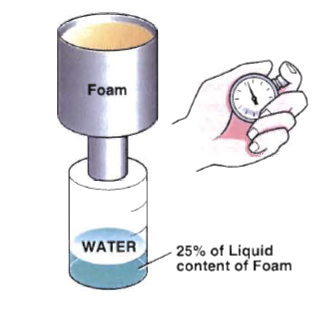
\includegraphics[width=\textwidth]{drainage_test.png}
    \caption{}
\end{subfigure}

\caption{a) Low expansion test and b) drainage test \cite{aamodt2020review}.}
\label{ch2:figure:tests}
\end{figure}

Researchers have been working on optimizing the foaming ability, hence the stability of foams, particularly for low expansion foams.  An experimental work to analyze and compare the drainage time and bubble size distribution of various firefighting foams was described by Mark et al \cite{laundess2012suppression}. Table \ref{ch2:table:times} shows the results of \cite{laundess2012suppression} comparing the 25\% of drainage times at an expansion ratio of 7:1 for two different foam concentrates. \\

\begin{table}[H]
\caption{Comparison of 25\% drainage times at 7:1 expansion \cite{laundess2012suppression}.}   

\centering
\begin{tabularx}{\textwidth}{>{\hsize=1.1\hsize}X >{\hsize=1.1\hsize}X >{\hsize=.89\hsize}X >{\hsize=.89\hsize}X >{\hsize=.89\hsize}X >{\hsize=1.1\hsize}X}
    \hline
    \multicolumn{6}{c}{Mean Drainage time (s)} \\
    \hline
    Foam \allowbreak concentrate & Generation system & Mean & Max & Min & Standard \allowbreak Deviation \\ 
    Tolomet 6\% & ISNF & 342 & 450 & 264 & 93 \\
    & \acrshort{caf} & 488 & 533 & 430 & 53 \\
    & Aspirated & 197 & N/A & N/A & N/A \\
    FC-600 3\% & ISNF & 539 & 725 & 450 & 126 \\
    & \acrshort{caf} & 1060 & 1281 & 844 & 288 \\
    & Aspirated & 485 & N/A & N/A & N/A \\
    \hline
\end{tabularx}

\label{ch2:table:times}
\end{table}

The results indicate that drainage rates for the various foam types were quite different, which may be explained by differences in the bubble size distributions as discussed below in Figure \ref{ch2:figure:distributions}. To explain the differences in foam drainage rates between the three foam types, they studied the bubble size distributions for each foam type.

\begin{figure}[H]
    \centering
    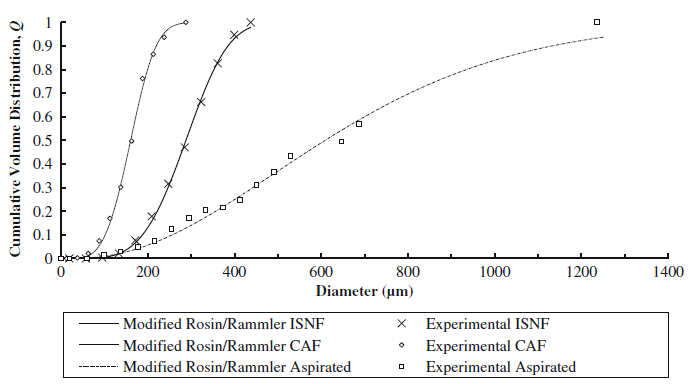
\includegraphics[width=\textwidth]{bubble_size_distributions.png}
    \caption{Cumulative bubble size distributions for various foam generation methods \cite{laundess2012suppression}.}
    \label{ch2:figure:distributions}
\end{figure}

As shown in Figure \ref{ch2:figure:distributions}, the drainage time is profoundly dependent upon the foam generation type. Also, the aspirated foam generation method produced larger bubbles in terms of size. These bubbles contributed to shorter drainage times as seen in Table \ref{ch2:table:times}, hence the reduction of foam quality and stability. This correlation technique used was benchmarked by \cite{oguike2013study} and most researchers have concluded the same as \cite{laundess2012suppression}. Mukunda and Dixit \cite{csb2016phenomenological} constructed a model of foam drainage based on momentum flux balance and conducted experiments with an apparatus with foam drainage through a fuel layer. Their results showed a linear relationship of 25\% drainage time with the height consistent with the theoretical expectations. A recommendation made by \cite{laundess2012suppression} indicates that there is a need for further research to develop a new surfactant formulations immune to the oxidation reaction that generates nitrogen bubbles. This foam generation method will simultaneously increase the drainage rates and stability of low expansion foams due to nitrogen bubbles.

\section{Critical application rates}
In the most recent decade, most researchers have been interested in the application rates of various firefighting foams. A number of studies on effective application rates have increased significantly and most of these studies have been based on protein and synthetic based foams. The underlying motivation for considering diverse critical application rates was to identify the compatibility of foams on various class of fires. With the original motivation behind the development of synthetic based foams being economic issues, the application rates were, thus critical.

Most of the research on firefighting foams are based on optimization aiming to provide the necessary effectiveness and efficiency in performance. The basis for the current minimum application rates was originally developed in 1972 by Geyer \cite{geyer1972evaluation} in tests of protein and \acrshort{afff} solutions. These were "modelling" tests with \acrfull{jp-4} pool fires that measured 21 m, 30 m, and 43 m in diameter. They also included large-scale verification tests with a B-47 aircraft and simulated shielded fires, conducted with \acrshort{jp-4} pool fires 34 m and 43 in diameter with all tests conducted using air-aspirating foam generation method. The outcomes by \cite{geyer1972evaluation} showed that PF and \acrshort{afff} have an application rate with a ratio of 1.49:1 respectively and is shown in Figure \ref{ch2:figure:pool}. This difference in application rate recognizes the inherent advantage of using \acrshort{afff} to extinguish hydrocarbon pool fires and reflects the fact that \acrshort{afff} has been demonstrated to extinguish pool fires more rapidly than PF at equivalent application rates. For equivalent extinguishment times, lower rates of \acrshort{afff} than PF are required \cite{scheffey1995evaluating}.

\begin{figure}[H]
    \centering
    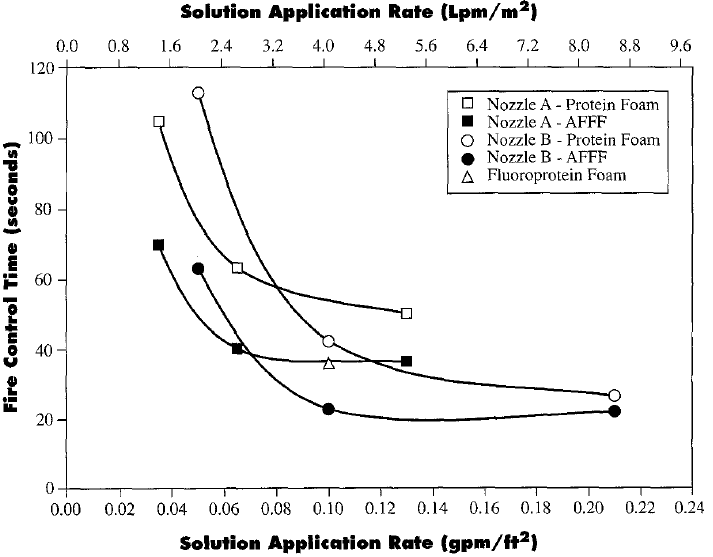
\includegraphics[width=\textwidth,height=11cm]{fire_control_time_pool_fires.png}
    \caption{Fire control time as a function of solution application rate using protein foam and \acrshort{afff} on \acrshort{jp-4} pool fires \cite{geyer1972evaluation}.}
    \label{ch2:figure:pool}
\end{figure}

Numerous experimental tests have been conducted by many researchers with purpose of validating these application rates. Geyer et al \cite{geyer1979comparative} further conducted tests on critical application rates for validation. The experimental tests conducted were focused on fire control time as a function of solution application rate for PF, AFF, and FPF for Jet A fuel fires and the results are shown in Figure \ref{ch2:figure:fuel}. These were aiming in employing more foam generation methods and different fire type to make necessary analyses of outcomes and compare with \cite{geyer1972evaluation}. Based on Figure \ref{ch2:figure:pool} and \ref{ch2:figure:fuel}, the application rate is greatly dependent on the type of foam generation and also the type of foam concentrates utilised. There have been numerous challenges regarding the critical applications of firefighting foams. The proliferation of performance guidelines and specifications for firefighting foams has created divergent opinions especially on aviation industry fire protection standards \cite{scheffey1995evaluating}.

\begin{figure}[H]
    \centering
    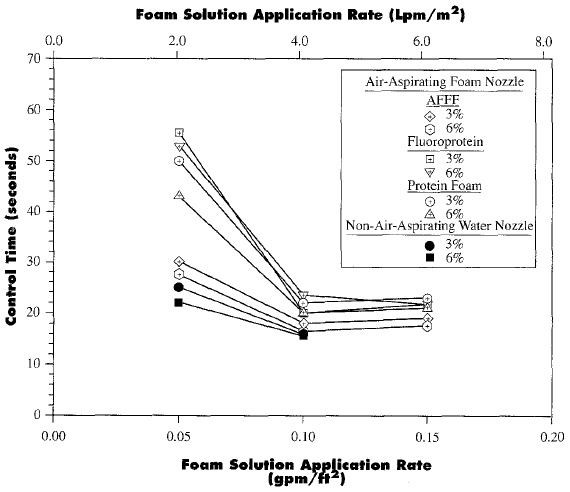
\includegraphics[width=\textwidth,height=11cm]{fire_control_time_fuel_fires.png}
    \caption{Fire control time as a function of solution application rate for \acrshort{afff}, fluoroprotein and protein foams for Jet A fuel fires \cite{geyer1972evaluation}.}
    \label{ch2:figure:fuel}
\end{figure}

\section{Effect of degradability}
Aircraft accidents are currently not a threatening issue in South Africa. This is due to a drastic decrease in air-crash over the past years. Nevertheless, fire protection in South African aviation has always been compliant. Due to this drastic decrease in air-crash, firefighting resources including firefighting foam last a long time without actually being realistically tested. Firefighting foams naturally degrade over time due to several factors such as liquid drainage driven by gravity and coarsening. Firefighting foam degradation is defined by Hinnant et al \cite{hinnant2017influence} as a reduction in foam layer thickness regardless of any changes in foam density or 'quality'.

In the present research work, it is essential to comprehend the impact of different storage facilities on foam degradation. In this way, advancing the storage facility focusing on degradation will be uncomplicated. Aviation periodic training is the only platform of testing foam performance parameters, hence foam degradation. As a result, it may not indicate the precise causes of degradation as this is not an actual situation. Foam's effectiveness can be severely deteriorated by foam degradation. Thus, foam degradation can be influenced by many factors including the hot fuel, fire, and foam formulation that contains surfactants and additives needed to generate the foam \cite{hinnant2017influence}. Although these factors are known, some of them such as fuel and fire cannot easily be controlled.    

During the firefighting process, foam is continuously interacting with fuel and flame. The interaction may immensely destroy the thick layer of the foam \cite{osei2015foam}. In this way, the ability of foam will be reduced, thus its performance may be compromised. However, foam degradation may suddenly increase dramatically during this process.  The causes for this are not well understood due to the lack of research on foam degradation. Furthermore, the individual effect of fire and fuel on degradation are inseparable due to the presence of fire \cite{hinnant2017influence}. 

Previous research on foam degradation has mostly focused on the natural aging process of foam \cite{do2011numerical} and the effect of the interaction of hydrocarbon liquids with foam \cite{osei2015foam}.  The natural aging of foam can be mainly influenced by the storage tank utilized, which is essential in this research work as the optimization of the storage facility based on degradation will be benchmarked by these previous Research. Hinnant et \cite{hinnant2017influence} studied the influence of fuel on foam degradation for fluorinated and fluorine-free foams. The study outcome showed that the fuel temperature is by far the major factor contributing to foam degradation followed by the effects of surfactant formulation, type of fuel, and bubble diameter or expansion ratio. Figure \ref{ch2:figure:degradation} shows the percentage change in \acrshort{afff} thickness versus time at room temperature, 35, 50, 75, and 90℃.

\begin{figure}[H]
    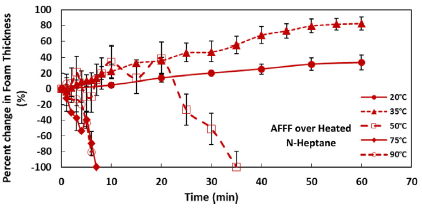
\includegraphics[width=.65\textwidth]{foam_degradation.png}
    \caption{\acrshort{afff} foam degradation versus time over n-heptane fuel at different temperatures \cite{hinnant2017influence}.}
    \label{ch2:figure:degradation}
\end{figure}

Parameters such as bubble diameter or expansion ratio are much dependent on the foam generation method, which is discussed in section 2.4. Larger bubbles cause a rapid drainage rate than smaller bubbles, and according to \cite{hinnant2017influence}, the increased drainage rate can cause the foam to degrade rapidly. In this way, the storage facility may indirectly affect foam degradation. This is due to the sediments or sludge, which may accumulate in the storage facility during the aging process. Consequently, sediments may affect foam characteristics, particularly bubble distribution during the foam generation process, this is shown by employing a flow process in Figure \ref{ch2:figure:effect}. The optimization of a storage facility in reducing the accumulation of sediments will prove to extensively reduce foam degradation.

\begin{figure}[H]

\centering
\begin{adjustbox}{center}
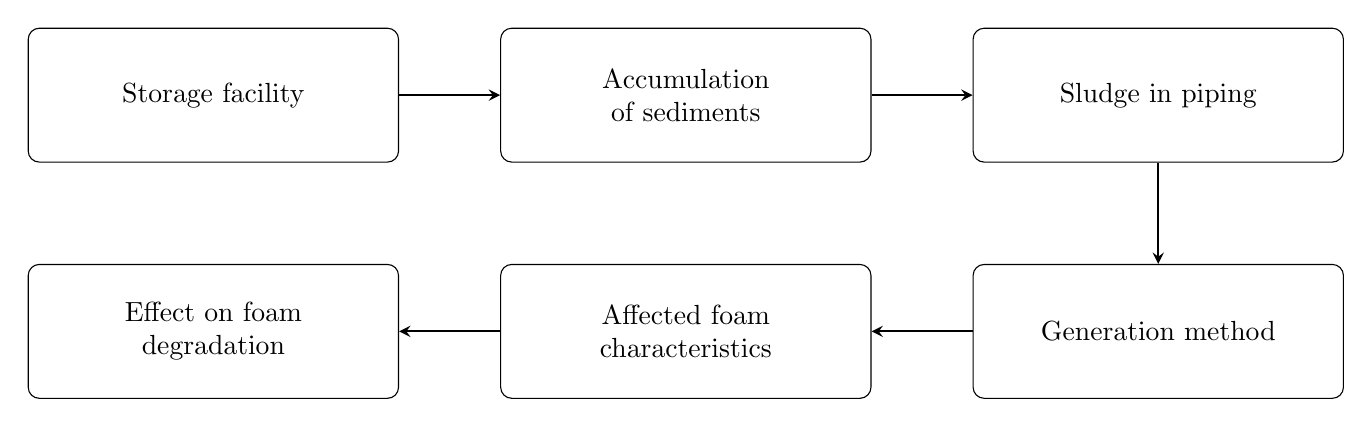
\begin{tikzpicture}[node distance=6cm]
    \tikzstyle{block} = [rectangle, rounded corners, draw, text centered, text width=4cm, inner sep=1em, minimum height=1.7cm]
    \tikzstyle{arrow} = [thick,->,>=stealth]

    \node (storage) [block] {Storage facility};
    \node (accumulation) [block, right of=storage] {Accumulation of sediments};
    \node (sludge) [block, right of=accumulation] {Sludge in piping};
    \node (generation) [block, below of=sludge, yshift=3cm] {Generation method};
    \node (affect) [block, left of=generation]{Affected foam characteristics};
    \node (effect) [block, left of=affect] {Effect on foam degradation};

    \draw [arrow] (storage) -- (accumulation);
    \draw [arrow] (accumulation) -- (sludge);
    \draw [arrow] (sludge) -- (generation);
    \draw [arrow] (generation) -- (affect);
    \draw [arrow] (affect) -- (effect);
\end{tikzpicture}
\end{adjustbox}

\caption{Effect of \acrshort{afff} degradation.}
\label{ch2:figure:effect}
\end{figure}

There have been fewer studies on the effect of surfactant formulation on degradation, further research should be conducted to detect the effect of this parameter on foam degradation. Furthermore, other parameters that may affect foam degradation should be extensively investigated in the future as foam degradation may regularly affect the performance of the foam.

\section{Environmental issues}
Modern firefighting foams can be considered as sensational in terms of physical characteristics, but, in recent years, the new Registration Evaluation Authorization and Restriction of Chemicals (REACH) legislation have drawn attention to their ecotoxicological properties \cite{turekova2011environmental}. While \acrshort{afff} is the most widely used firefighting foam in aviation fire protection, it still has some disadvantages, of which one of those is the environmental impact \cite{zhao2016improving}. Due to growing concerns regarding the impact that firefighting foams have on the environment, steps need to be taken to rectify this situation. To date, few papers have looked at the environmental impact of \acrshort{afff}. This lack of research on environmentally friendly surfactants must be addressed with more experimental studies to reduce the contamination of the environment, especially in aviation industry.

Although \acrshort{afff} has numerous advantages over other firefighting foams, their environmental issues have been a huge setback. Initially, \acrshort{afff} contained substances such as perfluoroalkyl and poly-fluoroalkyl (PFAS). Previous research shows that PFAS had significantly caused the contamination of soil, groundwater, and surface water including water stream animals as a result of \acrshort{afff} being released during aviation periodic training \cite{milley2018estimating}. As shown in Figure \ref{ch2:figure:use}, this poses acts of negligence and is hazardous to the environment as foam detoxifies naturally in soil.

\begin{figure}[H]
    \centering
    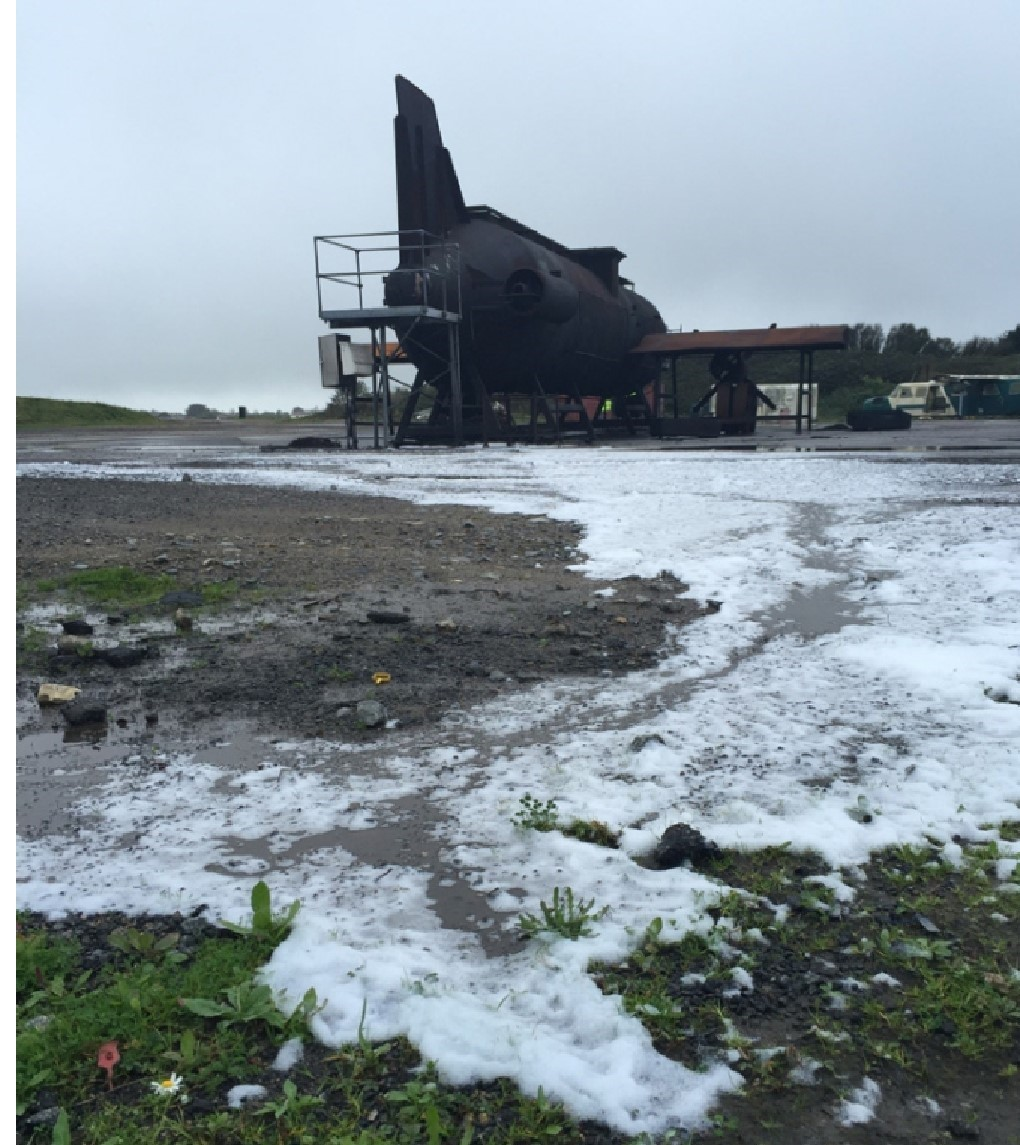
\includegraphics[width=\textwidth,height=9cm]{use_during_aviation_training.jpg}
    \caption{Used \acrshort{afff} during aviation periodic training.}
    \label{ch2:figure:use}
\end{figure}

Initially, PFAS's have not been previously known or recognized to be harmful in the environment. This was due to the complexity of \acrshort{afff} mixtures utilized and previous significant gaps in thorough comprehending of PFAS, including their toxicity, bioaccumulation, occurrence, transport, and transformation mechanisms \cite{milley2018estimating}. However, PFAS's impact in the environment was then recognized in the late 1990s and several jurisdictions offered guidance with a limited range or amount of PFAS's that can impact the environment \cite{hinnant2017influence}.

Elimination of PFAS in \acrshort{afff} was a challenge for every manufacturer and aviation industries as these chemical substances were key during fire suppression. \acrshort{afff} was able to suppress fire rapidly due to the presence of PFAS's. With environmental regulations enforcing the elimination of PFAS, manufacturers had no other alternative but to cooperate in the elimination of PFAS's. Consequently, PFAS's were phased out in 2002 by all the manufacturers due to the environmental impact \cite{persson2003foamspex}.  Fluorinated surfactants replaced PFAS's instantly intending to reduce the environmental impact and still be compatible with \acrshort{afff}. 

According to the research, fluorinated surfactants were also found to have an impact on the environment \cite{martin2012fire}. As a result, samples that were analyzed in 2010 indicate that \acrshort{afff} manufacturers have commenced to gradually reduce or even eliminate fluorinated surfactants in their formulations \cite{milley2018estimating}. Moreover, this process of eliminating present surfactants is critical as the transition should be carefully analyzed, in order to prevent the possible negative influence, it might pose in the performance parameters of firefighting foam. To date, fluorinated surfactants are present in \acrshort{afff} and are continuously bio-persistent in the environment and pose health hazards to humans.

The main objective of the present research work is to improve the compatibility of the materials that are utilised to construct the storage facility. Therefore, the environmental issues of \acrshort{afff} are of significance in the present study, since the optimised storage materials should not negatively influence the composition of \acrshort{afff}, as this might then cause environmental issues during firefighting. 

In recent years, researchers have been investigating the effective ways of mitigating the environmental issues. While the progress of this optimization has been held back by the difficulties stated above. The \acrshort{nfpa} committee, which is responsible for \acrshort{nfpa} 11, \emph{low expansion foams}, has made significant effort in tasking a group to address the environmental concerns around low expansion foams \cite{scheffey1995evaluating}. The outcome of the task group has been recently published with a full guidance to end user\cite{scheffey1995evaluating}. Alternatively, researchers have managed to implement new surfactants which are environmentally friendly. However, commercial firefighting foams without fluorinated surfactants developed to date have not been able to extinguish the fire as rapid as \acrshort{afff} \cite{hinnant2017influence}. In the future, researchers will need to conduct an extensive investigation in order to implement the environmentally friendly surfactants that will be compatible with \acrshort{afff}.  

\section{Conclusions}
This chapter reviewed the relevant literature to gain a better and in-depth understanding of the various firefighting foams. The focus was diverted to \acrshort{afff}, where the evolution of this type of foam was studied. Various foam generation processes were discussed, and their impacts on the poor performance of \acrshort{afff}. Based on the previous studies, the aspirated nozzle is suitable for generating \acrshort{afff}. The equations involved during this process were analyzed, with some recommendations to optimize this process being detailed. The importance of the foaming ability and mechanical stability were addressed, and the findings of previous studies were discussed. It was then found that the stability directly affects the quality, hence the performance of the foam.

The next chapter evaluates the various engineering materials commonly used to construct the storage facility for \acrshort{afff} concentrate. It further investigates and recommends possible ways of enhancing the properties of these materials based on the current knowledge.